\section{Análisis de Constelaciones Propias}
% Se agrupa el trabajo de los 3 para ahorrar espacio y cumplir el límite de páginas.
Como parte de la validación del mapeo espacial en Envolvente Compleja, cada integrante del equipo diseñó una constelación inédita alterando el vector de la tabla de verdad. El objetivo fue observar cómo geometrías no convencionales reaccionan ante el Ruido Gaussiano Blanco Aditivo (AWGN) en comparación con el esquema estándar. Los diseños y sus vectores matemáticos se resumen en la Tabla \ref{tab:const_ineditas}.

\begin{table}[H]
    \centering
    \caption{Resumen de constelaciones propuestas por el equipo}
    \resizebox{\columnwidth}{!}{%
    \begin{tabular}{l l l}
        \toprule
        \textbf{Autor} & \textbf{Concepto Geométrico} & \textbf{Vector (I+Q) Seleccionado} \\
        \midrule
        Juan D. & Triángulo con punto central & $[0+1j, 0.8-0.5j, -0.8-0.5j, 0+0j]$ \\
        % [NOTA: Jordy y Valentina deben llenar sus filas aquí]
        Jordy & (Por definir) & $[...]$ \\
        Valentina & (Por definir) & $[...]$ \\
        \bottomrule
    \end{tabular}
    }
    \label{tab:const_ineditas}
\end{table}

\begin{figure}[H]
    \centering
    \subfloat[Diseño Juan D.]{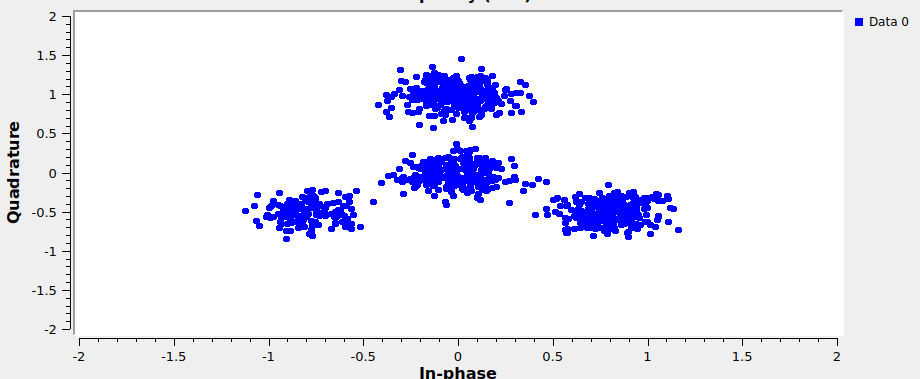
\includegraphics[width=0.32\linewidth]{imagenes/constelacion_creada.png}\label{fig:cj}}
    %\hfill
    % [NOTA: Jordy y Valentina deben cambiar "imagen_vacia.png" por los nombres de sus capturas]
    %\subfloat[Diseño Jordy]{\includegraphics[width=0.32\linewidth]{imagen_vacia.png}\label{fig:cjo}}
    %\hfill
    %\subfloat[Diseño Valentina]{\includegraphics[width=0.32\linewidth]{imagen_vacia.png}\label{fig:cva}}
    \caption{Dispersión de los símbolos para las constelaciones propuestas bajo canal AWGN.}
    \label{fig:constelaciones_equipo}
\end{figure}

A partir de los resultados gráficos (Figura \ref{fig:constelaciones_equipo}), se concluye que alterar la simetría del esquema PSK tiene un impacto directo en la probabilidad de error. Por ejemplo, en el diseño de Juan David, al ubicar un símbolo exactamente en el origen ($0+0j$), este requiere nula potencia pico de transmisión, pero su distancia euclidiana respecto a los otros tres símbolos se reduce drásticamente. Como se observa en la dispersión, la "nube" central está mucho más expuesta a solaparse; un ligero aumento en la varianza del ruido del canal causaría errores de decisión inmediatos en el receptor.

% [NOTA: Aquí agregarán sus conclusiones Jordy y Valentina sobre qué le pasó a sus propios diseños]